\section{Informal Logic Proof}

\subsection{ No Repeat }
The ``No Repeat Principle'' is formally proved in the Chao-Hong Chen's paper [1].
Here is the definition of the principle:
Given a reversible abstract machine and an initial state, for two different natural numbers m and n, if the initial state reach $st_{m}$ and $st_{n}$ by walking through m and n steps respectively, then $st_{m}$ should not beequal to $st_{n}$.

\subsection{ Narrow RevTerminate Principle }
Restating the statement of Narrow RevTerminate Principle: 
``Given a reversible abstract machine with a finite number of total states, it will inevitably terminate from any initial state.''

Here is the graph of the expected machine.  It seems monotonous: the initial state will traverse all the other states without repetition and then terminate.

\vspace{1em}

\usetikzlibrary{graphs, positioning, quotes, shapes.geometric}

\begin{document}
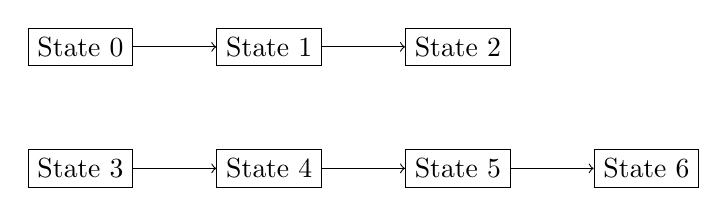
\begin{tikzpicture}[node distance=10pt]
    % 單純一條線,從initial state 到 finite state
    \node[draw]                           (State 0)  {State 0};
    \node[draw, right=30pt of State 0]    (State 1)  {State 1};
    \node[draw, right=30pt of State 1]    (State 2)  {State 2};
    
    \node[draw, below=30pt of State 0]    (State 3)  {State 3};
    \node[draw, right=30pt of State 3]    (State 4)  {State 4};
    \node[draw, right=30pt of State 4]    (State 5)  {State 5};
    \node[draw, right=30pt of State 5]    (State 6)  {State 6};

    \graph{
        (State 0) -> (State 1) -> (State 2);
        (State 3) -> (State 4) -> (State 5) -> (State 6);
    };
\end{tikzpicture}

This is the other case for the machine with finite states.  
In the graph, the initial state also traverses a finite number of states and terminates.  However, not all the states are traversed.

\vspace{1em}

\usetikzlibrary{graphs, positioning, quotes, shapes.geometric}

\begin{document}
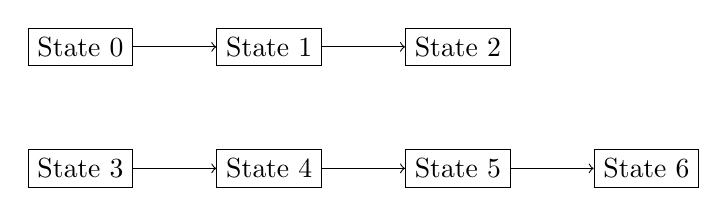
\begin{tikzpicture}[node distance=10pt]
    % 單純一條線,從initial state 到 finite state
    \node[draw]                           (State 0)  {State 0};
    \node[draw, right=30pt of State 0]    (State 1)  {State 1};
    \node[draw, right=30pt of State 1]    (State 2)  {State 2};
    
    \node[draw, below=30pt of State 0]    (State 3)  {State 3};
    \node[draw, right=30pt of State 3]    (State 4)  {State 4};
    \node[draw, right=30pt of State 4]    (State 5)  {State 5};
    \node[draw, right=30pt of State 5]    (State 6)  {State 6};

    \graph{
        (State 0) -> (State 1) -> (State 2);
        (State 3) -> (State 4) -> (State 5) -> (State 6);
    };
\end{tikzpicture}

Assume the number of all states is 𝑁.  That is, we have $st_{0}$, $st_{1}$, ..., and $st_{𝑁-1}$.
Assume $st_{0}$ is the initial state.  We can check whether $st_{0}$ has a next state.
Once the current state doesn't have next state, the machine will terminate.  
Therefore, we only need to consider the states starting from $st_{0}$ always have its next state.

When the trace progresses 𝑁 times, it should look like the graph below:

\vspace{1em}

\usetikzlibrary{graphs, positioning, quotes, shapes.geometric}

\begin{document}
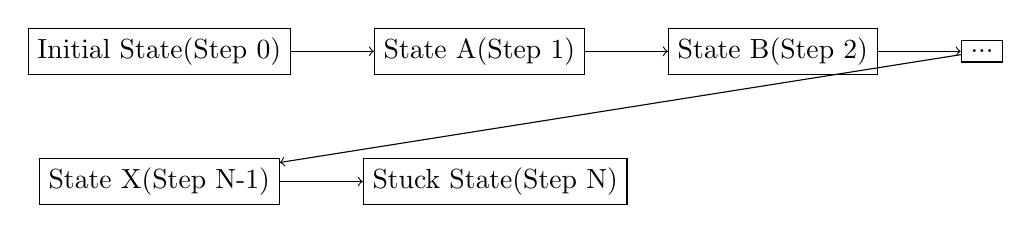
\begin{tikzpicture}[node distance=10pt]
    \node[draw]                           (State 0)  {Initial State(Step 0)};
    \node[draw, right=30pt of State 0]    (State 1)  {State A(Step 1)};
    \node[draw, right=30pt of State 1]    (State 2)  {State B(Step 2)};
    \node[draw, right=30pt of State 2]    (State 3)  {...};
    \node[draw, below=30pt of State 0]    (State 4)  {State X(Step N-1)};
    \node[draw, right=30pt of State 4]    (State 5)  {Stuck State(Step N)};
    
    \graph{
        (State 0) -> (State 1) -> (State 2) -> (State 3) -> (State 4) -> (State 5);
    };
\end{tikzpicture}

Here, we don't specifically mention that the first 𝑁 states traversed should be entirely non-repetitive, even though it's evident that a repetition would lead to a contradiction. 
Instead, we focus on the whole trace with a lenth of 𝑁 + 1.
The reversible machine has only 𝑁 states, but there are 𝑁 + 1 state we have traversed.
According to piegonhole principle, we can find two identical states in the trace.

\vspace{1em}

\usetikzlibrary{graphs, positioning, quotes, shapes.geometric}

\begin{document}
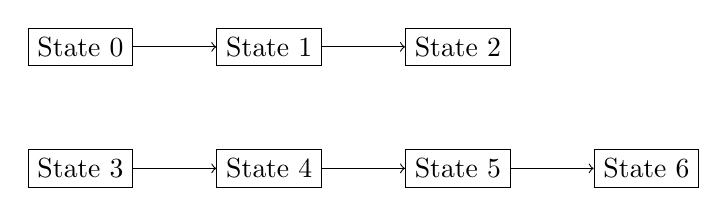
\begin{tikzpicture}[node distance=10pt]
    % 單純一條線,從initial state 到 finite state
    \node[draw]                           (State 0)  {State 0};
    \node[draw, right=30pt of State 0]    (State 1)  {State 1};
    \node[draw, right=30pt of State 1]    (State 2)  {State 2};
    
    \node[draw, below=30pt of State 0]    (State 3)  {State 3};
    \node[draw, right=30pt of State 3]    (State 4)  {State 4};
    \node[draw, right=30pt of State 4]    (State 5)  {State 5};
    \node[draw, right=30pt of State 5]    (State 6)  {State 6};

    \graph{
        (State 0) -> (State 1) -> (State 2);
        (State 3) -> (State 4) -> (State 5) -> (State 6);
    };
\end{tikzpicture}

With No-Repeat Principle, we know it's impossible for an initial state to walk through two different steps but reach same state.
At this point, we have successfully identified a contradiction.  
The contradiction shows that the length of trace is always less or equal than N, and thus the machine will terminate.

\subsection{ Broad RevTerminate Principle }
Restating the statement of Broad RevTerminate Principle: 
``Given a reversible abstract machine, it will inevitably terminate from any initial state with a finite number of reachable states.''

Similar to Narrow RevTerminate Principle, we assume $st_{0}$ is the initial state, and focus on the fact that there are always subsequent states after each state we traverse.
The Broad RevTerminate Principle asserts that there are a finite number of states $st_{0}$ can reach. 
Assume the number of reachable states from $st_{0}$ is 𝑁.
As before, we walk 𝑁 steps, making the length of the trace 𝑁 + 1.

\vspace{1em}

\usetikzlibrary{graphs, positioning, quotes, shapes.geometric}

\begin{document}
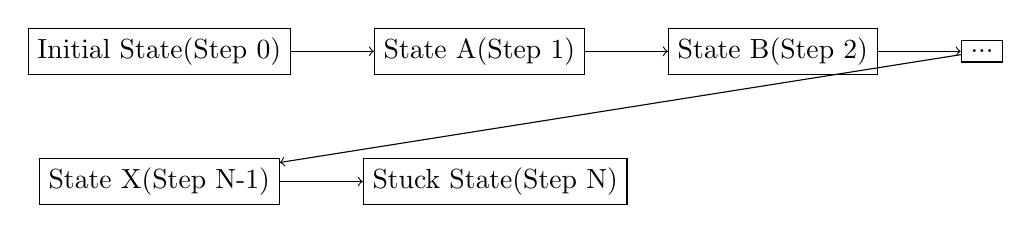
\begin{tikzpicture}[node distance=10pt]
    \node[draw]                           (State 0)  {Initial State(Step 0)};
    \node[draw, right=30pt of State 0]    (State 1)  {State A(Step 1)};
    \node[draw, right=30pt of State 1]    (State 2)  {State B(Step 2)};
    \node[draw, right=30pt of State 2]    (State 3)  {...};
    \node[draw, below=30pt of State 0]    (State 4)  {State X(Step N-1)};
    \node[draw, right=30pt of State 4]    (State 5)  {Stuck State(Step N)};
    
    \graph{
        (State 0) -> (State 1) -> (State 2) -> (State 3) -> (State 4) -> (State 5);
    };
\end{tikzpicture}

There are 𝑁 + 1 states we have traversed.  However, there are only N states $st_{0}$ can reach.
According to piegonhole principle, we can find two identical states in the trace.

\vspace{1em}

\usetikzlibrary{graphs, positioning, quotes, shapes.geometric}

\begin{document}
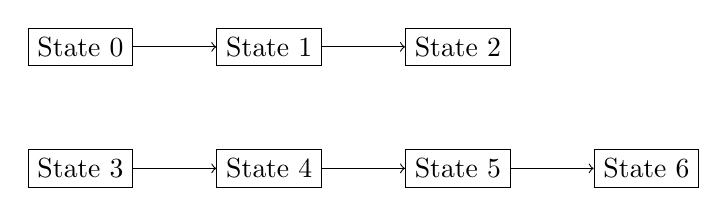
\begin{tikzpicture}[node distance=10pt]
    % 單純一條線,從initial state 到 finite state
    \node[draw]                           (State 0)  {State 0};
    \node[draw, right=30pt of State 0]    (State 1)  {State 1};
    \node[draw, right=30pt of State 1]    (State 2)  {State 2};
    
    \node[draw, below=30pt of State 0]    (State 3)  {State 3};
    \node[draw, right=30pt of State 3]    (State 4)  {State 4};
    \node[draw, right=30pt of State 4]    (State 5)  {State 5};
    \node[draw, right=30pt of State 5]    (State 6)  {State 6};

    \graph{
        (State 0) -> (State 1) -> (State 2);
        (State 3) -> (State 4) -> (State 5) -> (State 6);
    };
\end{tikzpicture}

With No-Repeat principle, we know it's impossible for an initial state to traverse two different steps and reach the same state.
At this point, we have successfully identified a contradiction.  The contradiction shows the length of trace is always less or equal than N, leading to termination.

